\documentclass[11pt, a4paper]{article}
%\usepackage{geometry}
\usepackage[inner=1.5cm,outer=1.5cm,top=2.5cm,bottom=2.5cm]{geometry}
\pagestyle{empty}
\usepackage{graphicx}
\usepackage{fancyhdr, lastpage, bbding, pmboxdraw}
\usepackage[usenames,dvipsnames]{color}
\definecolor{darkblue}{rgb}{0,0,.6}
\definecolor{darkred}{rgb}{.7,0,0}
\definecolor{darkgreen}{rgb}{0,.6,0}
\definecolor{red}{rgb}{.98,0,0}
\usepackage[colorlinks,pagebackref,pdfusetitle,urlcolor=darkblue,citecolor=darkblue,linkcolor=darkred,bookmarksnumbered,plainpages=false]{hyperref}
\renewcommand{\thefootnote}{\fnsymbol{footnote}}

\pagestyle{fancyplain}
\fancyhf{}
\lhead{ \fancyplain{}{Introduction to Data-Driven Healthcare} }
%\chead{ \fancyplain{}{} }
\rhead{ \fancyplain{}{Fall 2018} }
%\rfoot{\fancyplain{}{page \thepage\ of \pageref{LastPage}}}
\fancyfoot[RO, LE] {page \thepage\ of \pageref{LastPage} }
\thispagestyle{plain}

%%%%%%%%%%%% LISTING %%%
\usepackage{listings}
\usepackage{caption}
\DeclareCaptionFont{white}{\color{white}}
\DeclareCaptionFormat{listing}{\colorbox{gray}{\parbox{\textwidth}{#1#2#3}}}
\captionsetup[lstlisting]{format=listing,labelfont=white,textfont=white}
\usepackage{verbatim} % used to display code
\usepackage{fancyvrb}
\usepackage{acronym}
\usepackage{amsthm}
\VerbatimFootnotes % Required, otherwise verbatim does not work in footnotes!



\definecolor{OliveGreen}{cmyk}{0.64,0,0.95,0.40}
\definecolor{CadetBlue}{cmyk}{0.62,0.57,0.23,0}
\definecolor{lightlightgray}{gray}{0.93}



\lstset{
%language=bash,                          % Code langugage
basicstyle=\ttfamily,                   % Code font, Examples: \footnotesize, \ttfamily
keywordstyle=\color{OliveGreen},        % Keywords font ('*' = uppercase)
commentstyle=\color{gray},              % Comments font
numbers=left,                           % Line nums position
numberstyle=\tiny,                      % Line-numbers fonts
stepnumber=1,                           % Step between two line-numbers
numbersep=5pt,                          % How far are line-numbers from code
backgroundcolor=\color{lightlightgray}, % Choose background color
frame=none,                             % A frame around the code
tabsize=2,                              % Default tab size
captionpos=t,                           % Caption-position = bottom
breaklines=true,                        % Automatic line breaking?
breakatwhitespace=false,                % Automatic breaks only at whitespace?
showspaces=false,                       % Dont make spaces visible
showtabs=false,                         % Dont make tabls visible
columns=flexible,                       % Column format
morekeywords={__global__, __device__},  % CUDA specific keywords
}

%%%%%%%%%%%%%%%%%%%%%%%%%%%%%%%%%%%%
\begin{document}
\begin{center}
{\Large \textsc{Introduction to Data-Driven Healthcare}}
\end{center}
\begin{center}
Fall 2018
\end{center}
%\date{September 26, 2014}

\begin{center}
\rule{6in}{0.4pt}
\begin{minipage}[t]{.75\textwidth}
\begin{tabular}{llcccll}
\textbf{Instructors:} & Michoel Snow, MD PhD & & &  & \textbf{Time:} & F 8am - 10am \\
& Glen Ferguson, PhD &&&&& \\
\textbf{Email:} &  \href{mailto:msnow1@montefiore.org}{msnow1@montefiore.org} & & & & \textbf{Place:} & Mazer 5th floor conf room\\
& \href{mailto:glfergus@montefiore.org}{glfergus@montefiore.org}  &&&&& \\
\end{tabular}
\end{minipage}
\rule{6in}{0.4pt}
\end{center}
\vspace{.5cm}
\setlength{\unitlength}{1in}
\renewcommand{\arraystretch}{2}

\vskip.15in
\noindent\textbf{Course Description:} This course is an exploration of the modern healthcare informatics pipeline, highlighting core components within the context of real-world applications.  Through a mix of discussion and case based learning, each class will examine steps along the pipeline, how they fit into the larger informatics framework, as well as an analysis of their implementation based on real-world projects.  Some steps we will analyze include: clinical decision support, cohort selection, ethics of model building, artificial intelligence and machine learning within healthcare.  After completing this course students will be able to design complete informatics pipelines to use within their own research.  As the course progresses, students will be expected to present on components of informatics pipeline within their specific domains and opportunities for future informatics applications.  For the final project, teams of students will be expected to propose new domain-specific informatics pipelines.

\vskip.15in
\noindent\textbf{Prerequisites:} None

\vskip.15in
\noindent\textbf{Objectives:}  Students who complete the course in full, will be able to:
\begin{itemize}
	\setlength\itemsep{0em}
	\item Outline the components which form model bioinformatics pipelines
	\item Investigate possible hypotheses for clinical significance and system compliance
	\item Characterize hypotheses within the context of healthcare infrastructure 
	\item Identify stakeholders based on the scope of the project
	\item Identify sources of patient data and differentiate the various collection mechanisms/tools
	\item Develop a informatics driven research question
	\item Assess the quality of the generated data 
	\item Describe modeling frameworks to analyze the data 
	\item Contrast methods to evaluate the results of modeling
	\item Discuss methods of model implementation and care provider communication
	\item Design new data-driver pipelines for application within the healthcare system
\end{itemize} 

\vskip.15in
\noindent\textbf{Presentation and Grades:}
At the end of the course each group of students will present a novel tenable bioinformatics pipeline for use within the hospital or clinics.  The class is graded pass/fail based on in class participation and the final presentation. 


\pagebreak

\noindent \textbf{Tentative Course Schedule:}
\begin{enumerate}\setlength\itemsep{0em}
	\item Overview of course and introduction to buidling data driven bioinformatic pipelines
	\item Building clinical decision support systems (Implementation)
	\item Evaluating study results and model predictions (Modeling and Analysis) 
	\item Overview of machine learning models - part 1 (Modeling and Analysis)
	\item Overview of machine learning models - part 2 (Modeling and Analysis)
	\item Assessing data quality and preparing data for modeling and analysis (Data Preparation)
	\item Identifying data sources and implementing collection protocols (Data Collection)
	\item Calculating economic feasability and impact (Stakeholder concerns)
	\item Bioinformatics ethics and stakeholder engagement (Stakeholder Concerns)
	\item Healthcare administrative databases (Infrastructure)
	\item Exploratory data analysis (Hypothesis Generation)
	\item Small group presentations
\end{enumerate}

\vskip.3in
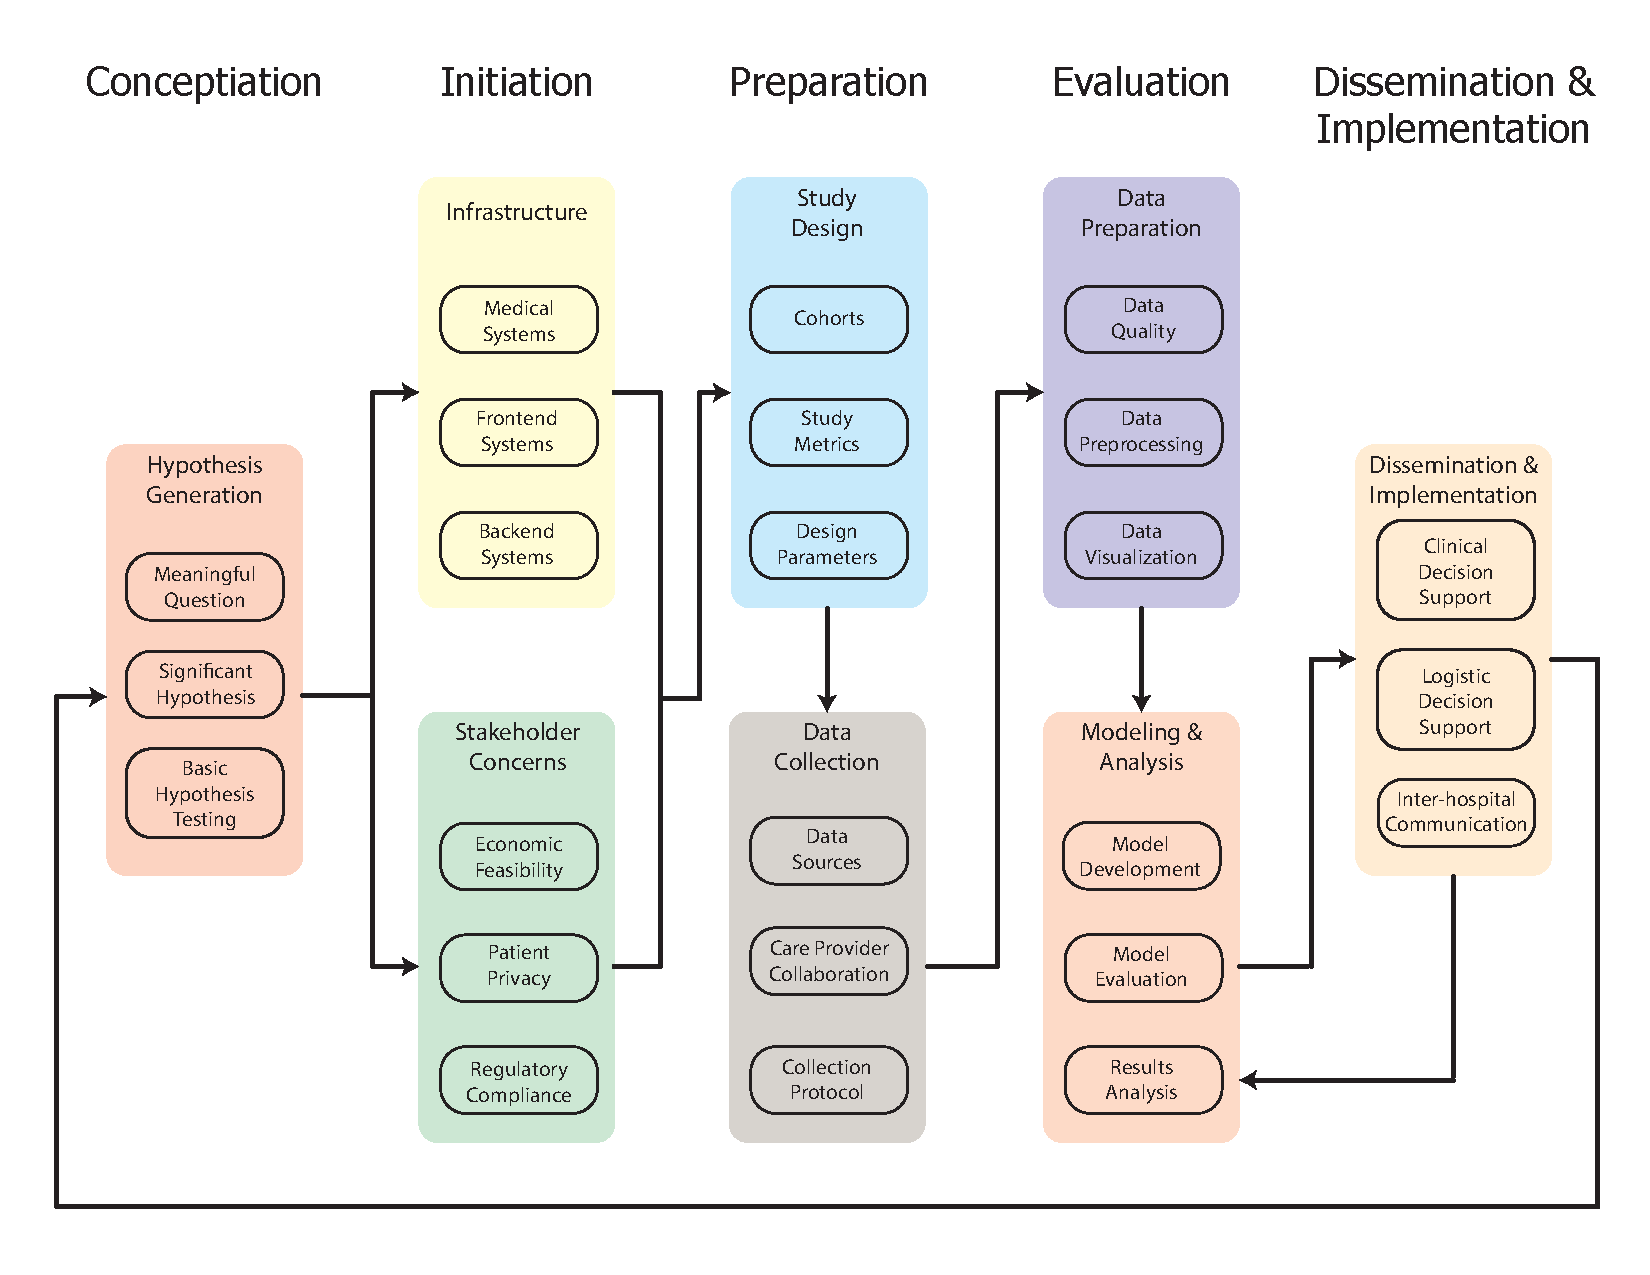
\includegraphics[width=0.9\textwidth]{informatics_pipeline.pdf}

%%%%%% THE END 
\end{document} 